\documentclass[10pt]{article}
\usepackage{longtable}
\usepackage{float}
\usepackage{wrapfig}
\usepackage{rotating}
\usepackage[normalem]{ulem}
\usepackage{amsmath}
\usepackage{textcomp}
\usepackage{marvosym}
\usepackage{wasysym}
\usepackage{amssymb}
\usepackage{hyperref}
\usepackage{color,soul} % for highlighting
\usepackage{graphicx}
\graphicspath{{/Users/benjaminbass/seacloud/class/earthMaterials/mineralSheets/tectosilicates/sanidine/images/}}

\usepackage{frame,color}
\usepackage{framed}
\usepackage{minibox}

% \usepackage[T1]{fontenc}
% \usepackage{tilting} %bring title up
% \setlength{\droptitle}{-10cm}

\usepackage[version=3]{mhchem}
% How to Use MChem
% \ce{SO4^2-}
% \ce{^{227}_{90}Th+}
% \ce{A\bond{-}B\bond{=}C\bond{#}D}
% \ce{CO2 + C -> 2CO}
% \ce{SO4^2- + Ba^2+ -> BaSO4 v}


\author{Benjamin Bass}
\date{24 February 2016}
\title{\vspace{-2.0cm}Sanidine} %bring title up temporary Fix

\begin{document}

\maketitle

% \framebox{Use frameboxes until figure out alignmen}

\begin{center}
  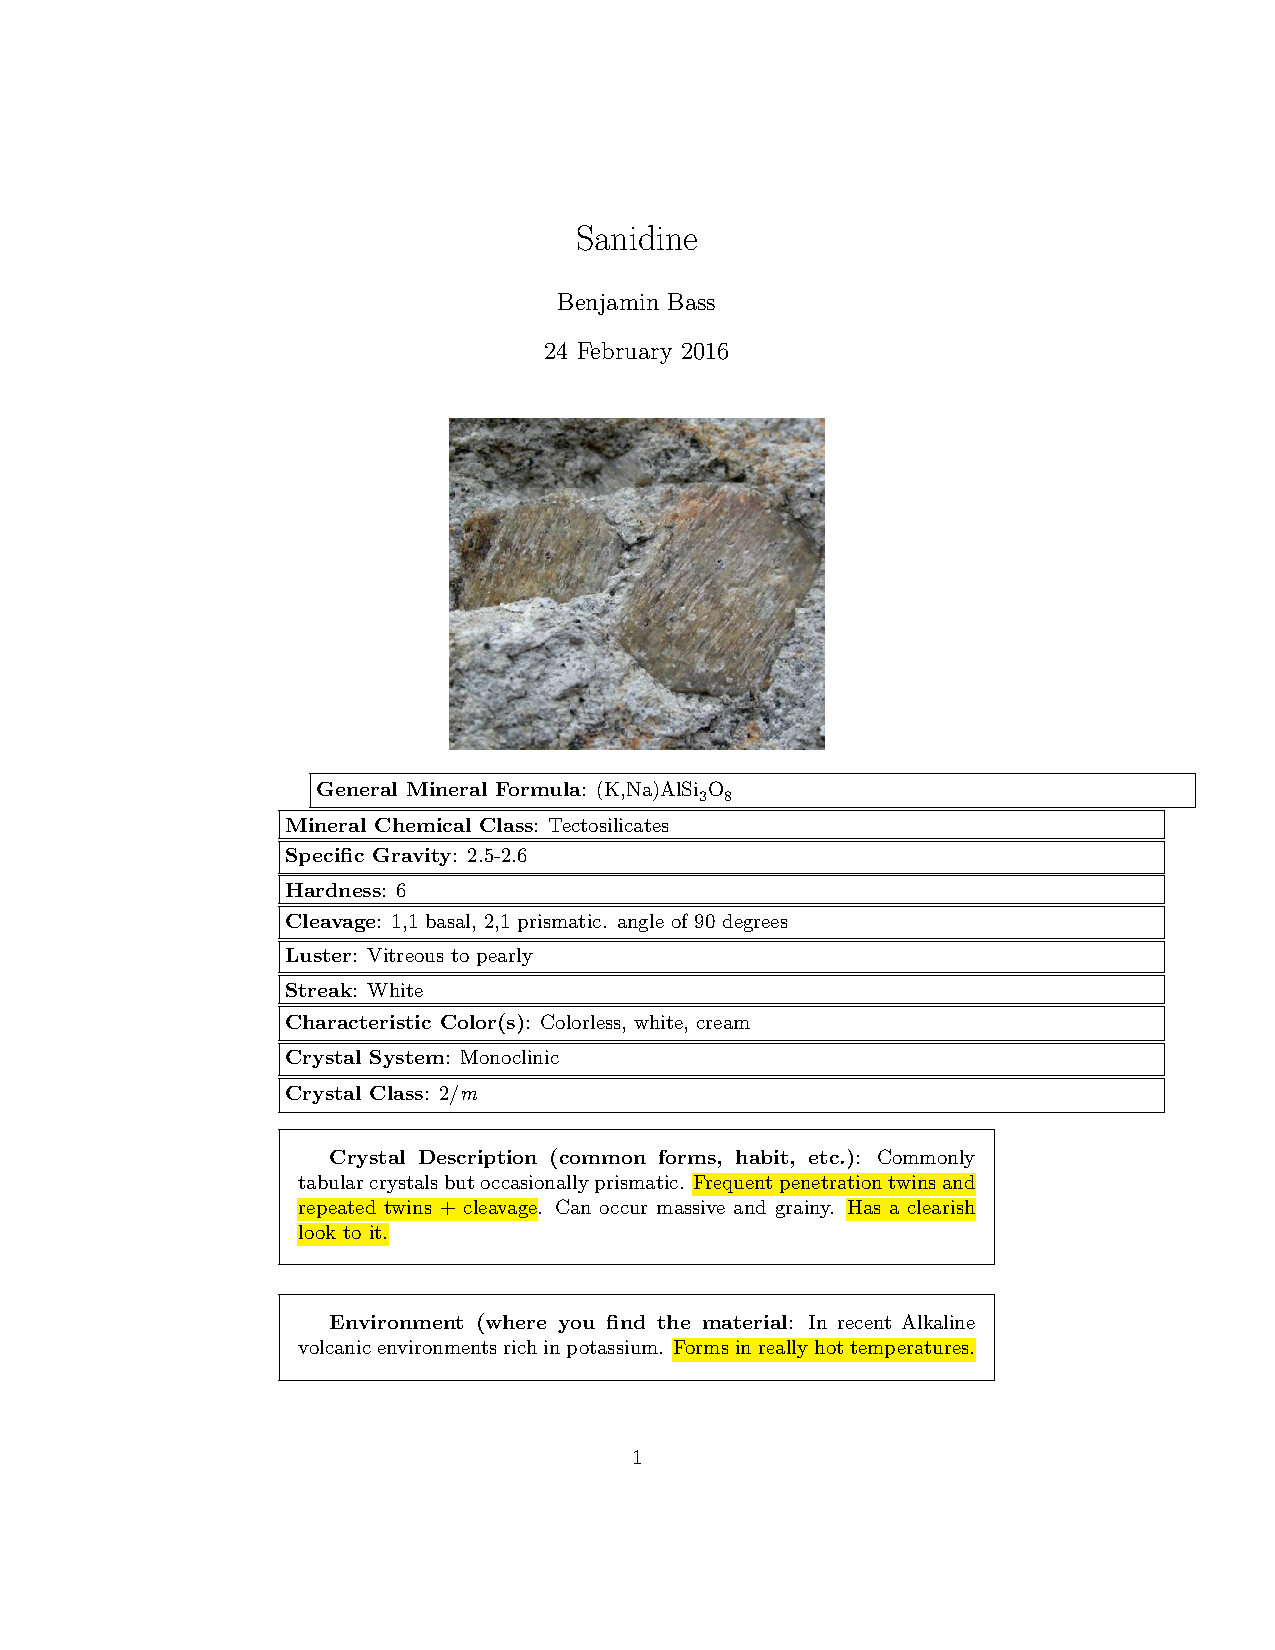
\includegraphics[scale=.4]{sanidine}
\end{center}



\framebox[15cm][l]{\textbf{General Mineral Formula}: \ce{ (K \text{,} Na)AlSi3O8 } }\
\framebox[15cm][l]{\textbf{Mineral Chemical Class}: Tectosilicates }\
\framebox[15cm][l]{\textbf{Specific Gravity}: 2.5-2.6 }\
\framebox[15cm][l]{\textbf{Hardness}: 6 }\
\framebox[15cm][l]{\textbf{Cleavage}: 1,1 basal, 2,1 prismatic. angle of 90 degrees }\
\framebox[15cm][l]{\textbf{Luster}: Vitreous to pearly }\
\framebox[15cm][l]{\textbf{Streak}: White }\
\framebox[15cm][l]{\textbf{Characteristic Color(s)}: Colorless, white, cream }\
\framebox[15cm][l]{\textbf{Crystal System}: Monoclinic }\
\framebox[15cm][l]{\textbf{Crystal Class}: 2/\it{m} }\

\begin{framed}
  \textbf{Crystal Description (common forms, habit, etc.)}: Commonly tabular crystals but occasionally prismatic. \hl{Frequent penetration twins and repeated twins + cleavage}. Can occur massive and grainy. \hl{Has a clearish look to it.}
\end{framed}

\begin{framed}
  \textbf{Environment (where you find the material}: In recent Alkaline volcanic environments rich in potassium. \hl{Forms in really hot temperatures.}
\end{framed}

\begin{framed}
  \textbf{Common Mineral Associations (in samples, also consult text, notes}: Quarts, muscovite, biotite, plag. feldspars, sodalite
\end{framed}

\begin{framed}
  \textbf{Scientific Usage/Significance}: None
\end{framed}

\begin{framed}
  \textbf{Industrial or Social Use/Significance}: Yellow variety used as a gemstone.
\end{framed}

\begin{framed}
  \textbf{Environmental Significance}: None
\end{framed}

% Possible other Solutions
% \framebox(300,20){\minibox{\textbf{R-Sq}:For example}}

\end{document}
%%% Local Variables:
%%% mode: latex
%%% TeX-master: t
%%% End:
